\section{实验论证}

\subsection{数据集}
本实验采用了MovieLens\footnote{\url{http://grouplens.org/datasets/movielens/}}100k的数据集.并随机分割了数据集的80\%作为训练数据, 其余20\%作为测试数据。

\textbf{MovieLens}包含了943个用户对于1682个电影的100,000个评分数据。每个用户至少对20个电影评过分。在实验中, 用户的职业信息(occupational description)被用作用户的内容信息(content information), 电影标题中的关键词被用作电影的内容信息。与\cite{gunawardana2009unified}中的处理过程相同, 我们并不直接使用用户的等级评分数据, 而将其转化为隐式反馈数据(对电影评过分为positive, 未评过分为negative)来使用, 以此推测是否用户是否会有对电影进行评分的行为。因此, 对于一个特定的用户而言, 我们的任务就是为其预测的一个有着潜在评分可能电影的排序列表。

如图\ref{gra6}所示, MovieLens中的用户所评分过电影数目显然呈长尾分布, 有422个近一半的用户所评分过的电影个数在区间$[20, 56]$中。
\begin{figure}[htbp]
	% caption放上面就会显示在图的上方,出现在下面就是出现在图的下方
	
	\begin{center}
		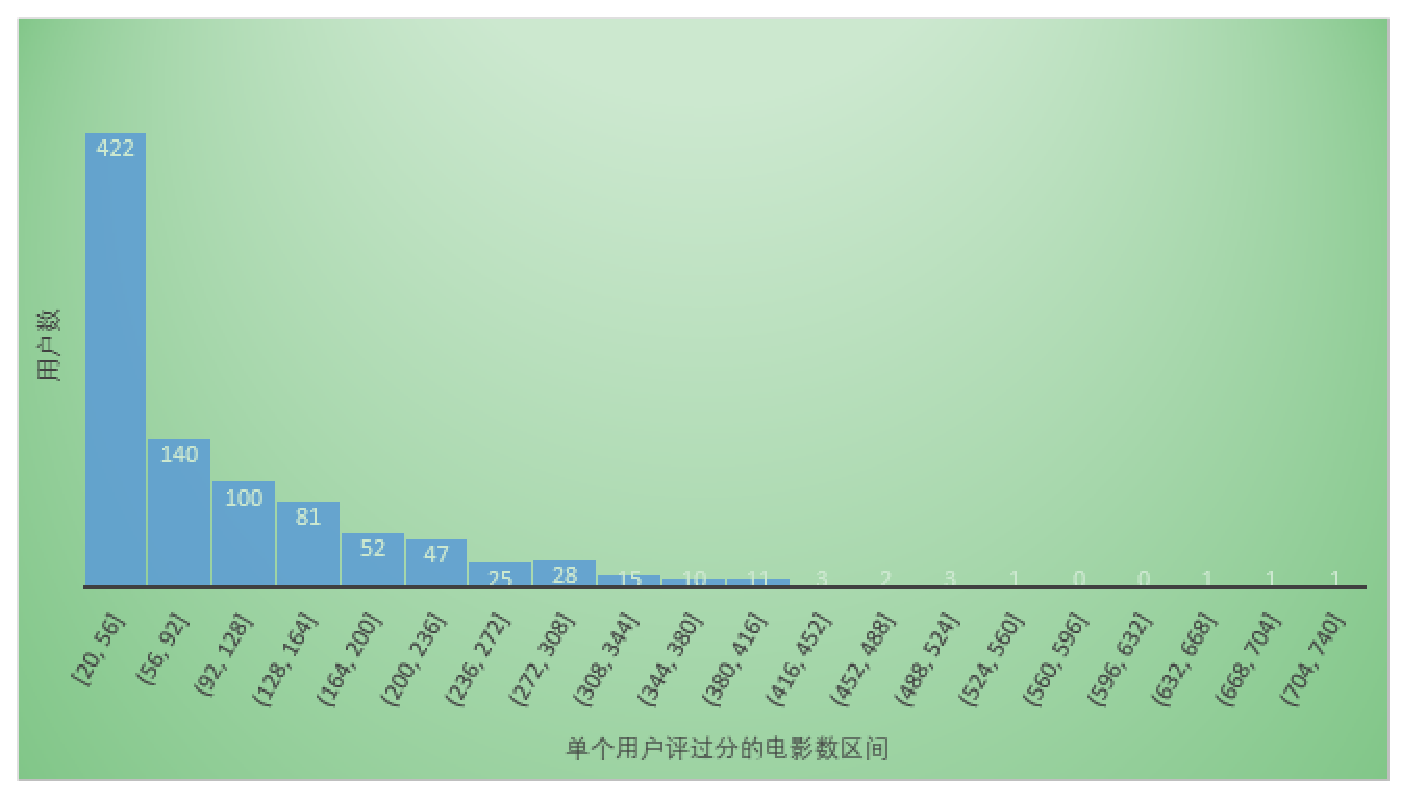
\includegraphics[width=5in]{longtail}
		\caption{用户对电影评分个数区间的长尾分布}
		\label{gra6}
	\end{center}
\end{figure}

\subsection{评测标准}

\textbf{MAP:} 对于$u$的平均准确率定义为:
\begin{equation*}
AP_u = \frac{1}{|\mathcal{I}_u^{te}|}\sum_{i \in \mathcal{I}_u^{te}}\left[\frac{1}{p_{ui}}\left(\sum_{j \in \mathcal{I}_u^{te}}\delta \left(p_{uj} \prec p_{ui}\right) + 1\right)\right]
\end{equation*}
在这里$p_{ui}$表示推荐列表中物品$i$的排序位置。$p_{uj} \prec p_{ui}$表示在对用户$u$的排序列表中物品$j$的排序位置在物品$i$的前面。
那么则有:
\begin{equation*}
MAP = \frac{\sum_{u \in \mathcal{U}^{te}}AP_u}{|\mathcal{U}^{te}|}
\end{equation*}


\textbf{NDCG:}
先从CG(Cummulative Gain)说起,  CG即将每个推荐结果相关性的分值累加后作为整个推荐列表的得分。
\begin{equation*}
CG_p = \sum_{i=1}^p rel_i
\end{equation*}
在$rel_i$表示处于位置$i$的推荐结果的相关性,$p$表示所要考察的推荐列表的大小

CG的一个缺点是没有考虑结果处于不同位置对结果的影响,例如我们总是希望相关性高的结果应排在前面,相关性低的结果排在靠前的位置会严重影响用户体验, 所以在CG的基础上引入位置影响因素,即DCG(Discounted Cummulative Gain):
\begin{equation*}
DCG_p = \sum_{i=1}^p \frac{2^{rel_i}-1}{\log_2 \left(i+1\right)}
\end{equation*}

DCG仍然有其局限之处,即不同的推荐列表之间,很难进行横向的评估。而我们评估一个推荐系统,不可能仅使用一个用户的推荐列表及相应结果进行评估, 而是对整个测试集中的用户及其推荐列表结果进行评估。 那么不同用户的推荐列表的评估分数就需要进行归一化,也即NDCG(Normalized Discounted Cummulative Gain)。

IDCG(Ideal DCG)为推荐系统某一用户返回的最好结果, 即假设返回结果按照相关性排序, 最相关的结果放在最前面, 此序列的DCG为IDCG。因此DCG的值介于 $(0,IDCG]$,故NDCG的值介于$(0,1]$.

对于用户$u$的NDCG@k定义为:
\begin{equation*}
NDCG_u@k = \frac{DCG_u@k}{IDCG_u}
\end{equation*}

那么,则有:
\begin{equation*}
NDCG@k = \frac{\sum_{u\in \mathcal{U}^{te}}NDCG_u@k}{|\mathcal{U}^{te}|}
\end{equation*}

\subsection{实验过程与分析}
我们对BPR-MF与CA-BPR分别就MAP与NDCG评测指标进行了比较。BPR-MF\cite{rendle2009bpr}应用了矩阵分解的BPR算法框架,同时采用均匀采样策略选取训练采样。表\ref{tab:characteristic}显示了试验方法的不同之处。
\begin{table}[htbp]
	\caption{BPR-MF与CA-BPR方法特征比较}
	\renewcommand\arraystretch{1.3}%改变行高
	\label{tab:characteristic}
	\begin{center}
		\begin{tabular}{|c|c|c|}
			
			\hline
			Method   &   Content & Sampling \\
			\hline
			\renewcommand\arraystretch{1}%改变行高
			BPR-MF   &   no      & uniform  \\
			CA-BPR   &   yes     & non-uniform\\
			\hline
			
		\end{tabular}
	\end{center}
\end{table}

表\ref{tab:mapandndcg}显示了BPR-MF与CA-BPR的MAP与NDCG实验结果。
\begin{table}[htbp]
	\caption{不同维度k下算法MAP与NDCG实验结果}
	\label{tab:mapandndcg}
	\begin{center}
		\begin{tabular}{|c | c |c |c|c|c|}
			\hline
			BPR-MF  &   k=10 &   k=20 &    k=30&    k=40&    k=50\\
			\hline
			MAP      &  0.0879&  0.0877&  0.1043&  0.0888&  0.1074\\
			\hline
			NDCG@3   &  0.3051&  0.3545&  0.3398&  0.2491&  0.3790\\
			NDCG@5   &  0.3616&  0.4296&  0.3708&  0.2984&  0.4153\\
			NDCG@10  &  0.4120&  0.4632&  0.4010&  0.3163&  0.4458\\
			NDCG@20  &  0.4121&  0.4575&  0.4164&  0.3415&  0.4323\\
			\hline
		\end{tabular}
		
		\begin{tabular}{|c | c |c |c|c|c|}
			\hline
			CA-BPR  &     k=10&   k=20 &    k=30&  k=40 &   k=50\\
			\hline
			MAP     &   0.1074&  0.1072&  0.1274&  0.1016&  0.1229\\
			\hline
			NDCG@3  &   0.3790&  0.4336&  0.4152&  0.3044&  0.4631\\
			NDCG@5  &   0.4153&  0.4752&  0.4531&  0.3646&  0.5074\\
			NDCG@10 &   0.4458&  0.5101&  0.4900&  0.3865&  0.5447\\
			NDCG@20 &   0.4323&  0.4946&  0.5088&  0.4173&  0.5282\\
			\hline
		\end{tabular}
	\end{center}
\end{table}

图\ref{fig:map}显示了BPR-MF与CA-BPR在不同维度下的MAP结果对比。
\begin{figure}[htbp]
	\begin{center}
	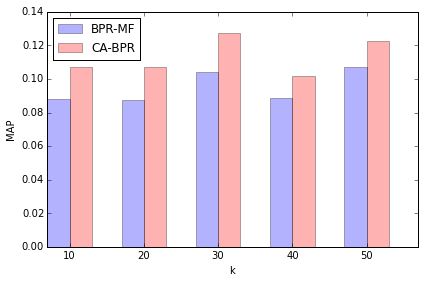
\includegraphics[width=4in]{mapbar}
\end{center}
\caption{不同维度算法MAP结果对比}
\label{fig:map}
\end{figure}
